\documentclass[10pt]{beamer}


\usetheme[progressbar=frametitle]{metropolis}
\usepackage{graphicx}
\usepackage{float}
\pagestyle{empty}
\usepackage{subcaption}
\usepackage{appendixnumberbeamer}
\usepackage{booktabs}
\usepackage[scale=2]{ccicons}
\usepackage{pgfplots}
\usepgfplotslibrary{dateplot}

\usepackage{xspace}
\newcommand{\themename}{\textbf{\textsc{metropolis}}\xspace}

\title{Genetic Algorithms}
\subtitle{Parameter Analysis}
 \date{\today}
%\date{2017-12-09}
\author{Yuri Lavinas}
\institute{University of Tsukuba}
% \titlegraphic{\hfill\includegraphics[height=1.5cm]{logo.pdf}}

\begin{document}

\maketitle



\begin{frame}{Parameter Analysis - GA}
	\begin{alertblock}{What is the best size for the tournament selection?}	
		Many work say $2$ (or a small value), but why?
	\end{alertblock}
	\begin{itemize}
		\item Exploitation X Exploration: No variation
		\item No recent experiments or theory
	\end{itemize}

	\begin{table}
		\begin{tabular}{|l|l|}
			\hline
			Papers with small values  & Papers	 explaining why \\ \hline
			13                                              & 0                                    \\ \hline
		\end{tabular}
	\end{table}
\end{frame}



\begin{frame}{Parameter Analysis - GA}
	\begin{alertblock}{Is $2$ really the best size for Tournament?}	
		We experimented many sizes on many benchmark functions
	\end{alertblock}
\begin{figure}
	\begin{subfigure}[b]{0.3\textwidth}
		\centering
		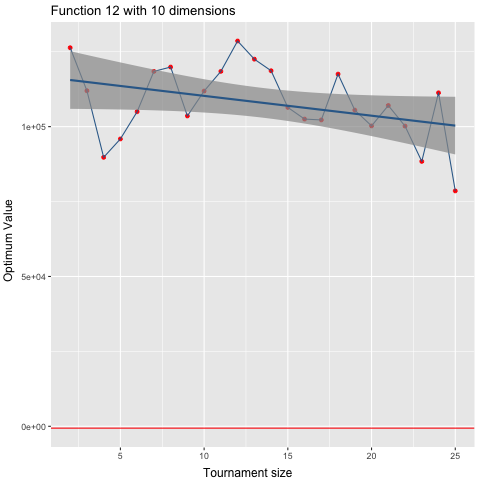
\includegraphics[width=\textwidth]{12dim_10.png}
		\caption{10 dimensions.}
	\end{subfigure}
	\begin{subfigure}[b]{0.3\textwidth}
		\centering
		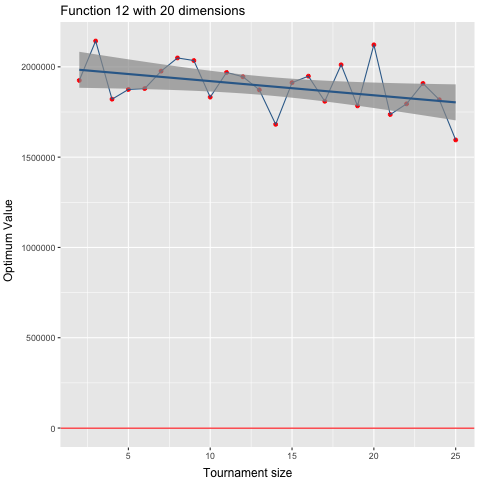
\includegraphics[width=\textwidth]{12dim_20.png}
		\caption{20 dimensions.}
	\end{subfigure}
	\begin{subfigure}[b]{0.3\textwidth}
		\centering
		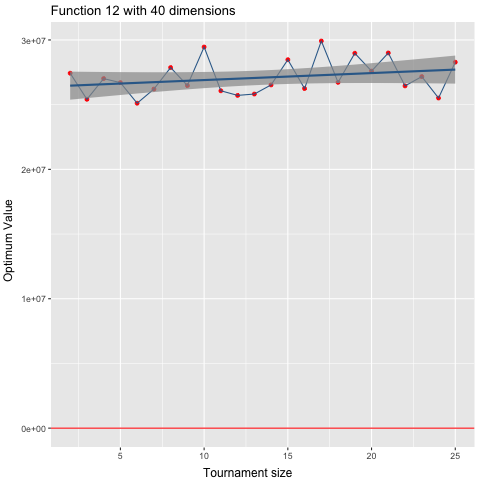
\includegraphics[width=\textwidth]{12dim_40.png}
		\caption{40 dimensions.}
	\end{subfigure}
	\caption{Average performance on different tournament size for the F12 function.}
	\label{12}
\end{figure}
\begin{itemize}
	\item But we could not find any strong relationship!
	\item Come to our poster to know more
\end{itemize}

\end{frame}

%\section{Questions?}
%
%
%{\setbeamercolor{palette primary}{fg=white, bg=black}
%\begin{frame}[standout]{}
%  Thank you!
%\end{frame}
%}
%


\end{document}

